La historia de la automoción comienza estrictamente en el siglo XIX.
Un automóvil es, por definición, un vehículo que se mueve a sí mismo
(del griego, \textit{αὐτός} ``a sí mismo'' y del latín \textit{mobilis},
``que se mueve'').

Desde los primeros modelos como la serie T, de Ford, hasta el inicio de
la fabricación de vehículos por parte de Mercedes Benz, la historia del
automovilismo ha estado llena de grandes logros y avances en un intervalo
de tiempo relativamente pequeño (figura \ref{fig:ford_model_t}):

\begin{figure}[H]
  \centering
  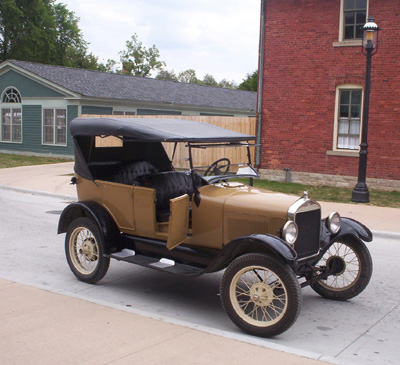
\includegraphics[width=.8\linewidth]{images/Late_model_Ford_Model_T.jpg}
  \caption{Ford modelo T del 1927 -- de Rmhermen \cite{Ford2022}.}
  \label{fig:ford_model_t}
\end{figure}

Durante aquella época, el ``mejor'' mecanismo de descubrimiento de
problemas era con algunos medidores y, sobre todo, por intuición:
sonidos del motor, olores extraños, \dots

No fue hasta los años 60 en donde los vehículos empezaron a incorporar
distintas interfaces con métricas que podían informar sobre el estado del
vehículo. El gran ``bum'' llegó con la expansión de la computadora, en donde
por primera vez se vio factible introducir un pequeño ordenador de 
abordo en el sistema.

En estos primeros sistemas, se incluyen indicadores del nivel de combustible,
sistema de refrigeración, presión del aceite, velocidad del motor,
temperatura del motor y otra información relativa al combustible. El
primer modelo que se conoce que incluye estos sistemas de cara a la
población en general es el Volkswagen Tipo III, en 1969 (figura \ref{fig:volkswagen_t3}):

\begin{figure}[H]
  \centering
  \includegraphics[width=.9\linewidth]{images/volkswagen_t3.jpg}
  \caption{Volkswagen Tipo III, modelo de inyección de 1969 -- de OSX - Trabajo propio \cite{VolkswagenTipo2021}.}
  \label{fig:volkswagen_t3}
\end{figure}

Pese a que supusieron un gran avance, estos primeros sistemas de
diagnóstico daban una información muy valiosa pero limitada, ya que muchos
diagnósticos seguirían siendo mediante los sentidos y las sensaciones
que le transmitiese el vehículo al mecánico. No fue hasta 1980 en donde
se implementó de forma estándar en los vehículos de \textit{General Motors}
el \ac{ALDL}, un lector de errores del coche que funcionó inicialmente a
160 baudios. Años más tarde, el sistema se refinaría usando el estándar
\ac{UART} \textit{half--duplex}, es decir, transmisión en los dos sentidos pero
no de forma simultánea (figura \ref{fig:aldl}). La principal motivación de incluir estos sistemas no fue
otra sino intentar reducir la contaminación de los vehículos teniendo
acceso a esta información \cite{SistemaOBD2Historia}.

\begin{figure}[H]
  \centering
  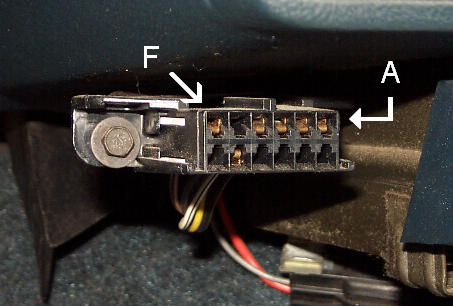
\includegraphics[width=.75\linewidth]{images/aldl.jpg}
  \caption{Conector \ac{ALDL}, creado por \textit{General Motors} antes de
  estandarizar OBD-II \cite{ReferenceManualChapter}.}
  \label{fig:aldl}
\end{figure}

No es hasta 1979 en que la \ac{SAE} recomienda crear un conector de
diagnóstico estandarizado en el mercado así como un conjunto de señales
de prueba. Finalmente, en 1991 la \ac{CARB} require que todos sus
vehículos tengan lo que sería el \ac{OBD}-I. Esta primera versión informaría
al conductor de un mal funcionamiento de alguno de los elementos del
vehículo mediante un \ac{MIL}, un indicador luminoso de fallos. Sin
embargo, solo se monitorizaban ciertos componentes relacionados con las
emisiones y no estaban calibrados \cite{SistemaOBD2Historia}.

Por ende, impulsado por las alertas \textit{smog} y por una fuerte regulación, en 1994
la \ac{CARB} obligó a todos los vehículos fabricados y vendidos a partir de 1996 incluir
el \ac{OBD}-II. Esto supuso un gran impulso en los mecanismos de monitorización de los
vehículos ya que además se estandarizó tanto el conector como los protocolos recomendados
por la \ac{SAE}. Tiempo más tarde, el Gobierno de los Estados Unidos aplicó la misma
medida a todos los vehículos del país \cite{SistemaOBD2Historia}.

Esta medida llegaría a Europa en 1998, según la Directiva 98/69EG, que obligaba a
todos los vehículos europeos a incluir dicho conector. Específicamente, los
automóviles de gasolina debían empezar a equiparlo en los modelos del año 2000; en el año 2003
para vehículos diésel; y en el año 2005 para camiones \cite{SistemaOBD2Historia}.

\subsection*{OBD--II}
\ac{OBD}--II es la segunda generación del sistema de diagnósticos de abordo, sucesor
de \ac{OBD}--I y su principal función es la de avisar al conductor cuando las
emisiones del vehículo son en torno a $1.5$ veces mayores de las diseñadas. A
diferencia de \ac{OBD}--I, \ac{OBD}--II también detecta fallos eléctricos, químicos
y mecánicos que puedan afectar al nivel de emisiones del vehículo (un caso típico
era un fallo químico del catalizador, indetectable por \ac{OBD}--I pero sí por la
segunda generación).

Este tipo de conector, al ser el primer estándar, cuenta con
múltiples interfaces que permiten conexiones mediante redes Wi-Fi, USB, Bluetooth,
etc. (cayendo pues en deshuso el protocolo de conexión por puerto serie -- RS232).
Esto se ha conseguido gracias al rápido avance de los sistemas embebidos, en donde
la combinación de \textit{software} y \textit{hardware} embebidos ha permitido que
cualquier usuario tenga acceso a este tipo de datos de forma relativamente simple
(actualmente, el conector más estandarizado es el controlador \texttt{ELM327} \cite{SistemaOBD2Historia},
figura \ref{fig:elm327}):

\begin{figure}[H]
  \centering
  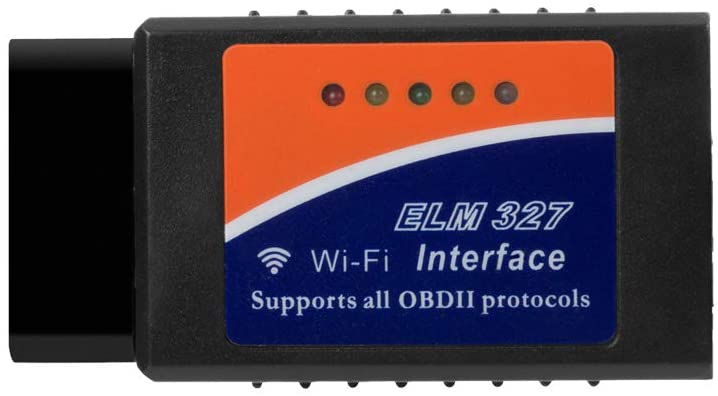
\includegraphics[width=.7\linewidth]{images/obd-ii-elm327.jpg}
  \caption{Controlador \texttt{ELM327} que cuenta con antenas Wi-Fi y Bluetooth para un acceso remoto \cite{AmazonComElm327}.}
  \label{fig:elm327}
\end{figure}

El sistema verifica todos los sensores directamente involucrados con las emisiones
del vehículo, como por ejemplo la inyección de aire al motor. Cuando algún sensor detecta
un fallo, se activa el \ac{MIL} indicando el fallo que sucede (o una combinación
de indicadores para notificar la existencia de un fallo, sin especificar exactamente
cuál).

El vehículo que incorpora un conector \ac{OBD}--II almacena la información sobre el
fallo del vehículo para que el mecánico que deba revisar el automóvil disponga de todos
los datos posibles. Por otra parte, este estándar permite una comunicación directa
con el vehículo mediante el envío de órdenes según un \ac{PID}. Por defecto, hay
una serie de \ac{PID}s estándar que la gran mayoría de vehículos deben incluir\footnote{%
Se dice ``la mayoría de vehículos'' porque hay ciertos \ac{PID}s que dependen
directamente del tipo de vehículo (a combustión, eléctrico, \dots) o del combustible
utilizado -- un vehículo eléctrico no ofrece información sobre las \ac{RPM} al igual
que un vehículo diésel no ofrece información sobre las bujías.}, pero también
los fabricantes de vehículos incluyen una serie de \ac{PID}s propios (conocidos como
\textit{\ac{PID}s propietarios}) que ofrecen información adaptada a cada vehículo
en particular y que, en principio, son privados y cerrados al público en general.

En Europa se implantó el \ac{EOBD}, la variación europea del estándar \ac{OBD}--II
implantada en el año 2000 en general. Si bien en apariencia es semejante al \ac{OBD}--II,
las diferencias radican en el \textit{software}. Por ejemplo, el estándar europeo
no monitoriza las evaporaciones del depósito de combustible; sin embargo, es más
sofisticado ya que usa ``mapas'' en las entradas de los sensores que obligan a que el
sensor se calibre empíricamente al sistema según las condiciones de operación del
motor (lo cual se traduce en que los sensores son mucho mejores pero más caros)
\cite{SistemaOBD2Historia}. Otra característica innovadora es que el sistema
europeo registra cuántos kilómetros se han recorrido desde que ha aparecido un
defecto \cite{EOBDOBD2}.

Finalmente, pero no menos importante, Japón tiene también su propio estándar denominado
\ac{JOBD}.

\subsection*{OBD--III}
El \ac{OBD}--III se espera que sea la siguiente versión del sistema que ya implementan
los coches actualmente. La principal diferencia con respecto a la versión anterior
será que el vehículo estará conectado de forma continua y emitiendo datos referentes
a las emisiones. De esta forma, se puede saber casi en el momento acerca de modificaciones
ilegales, un aumento en la contaminación del coche (signo de deterioro) y demás. No se
espera igualmente que sea un salto cualitativo ya que se sigue buscando que sea
altamente compatible con las herramientas que ya existen. Actualmente, se están
realizando pruebas en EE.UU. pero no hay cerrada ninguna fecha de estandarización
oficial por parte de los distintos continentes.

\subsection{Herramientas de monitorización y control del automóvil}
Pese al tiempo que lleva \ac{OBD}--II disponible, las herramientas existentes para
la actuación sobre un vehículo son relativamente escasas. La mayoría de modelos
presentes hoy en día en el mercado se basan directa o indirectamente en el
\texttt{ELM327}, un dispositivo de diagnóstico \ac{OBD} que cuenta con conexión
WiFi, Bluetooth y serie para la lectura local.

Por lo general, las herramientas que hay se utilizan por mecánicos o fanáticos del
sector para acceder a la información del estado del vehículo y ver los errores que
pudiera tener. Sin embargo, tras una breve documentación sobre el tema, la mayoría
de los casos buscaban directamente monitorizar en el momento el estado
del vehículo para obtener información relativa a los consumos, contaminación,
etc.

Por ejemplo, en el trabajo de Rimpas \textit{et al.} \cite{rimpasOBDIISensorDiagnostics2020}, se utiliza
un sensor \texttt{ELM327} para verificar que la información proporcionada por
el puerto del vehículo y la presentada por la telemetría presente en el mismo
(velocímetro y tacómetro) son coherentes entre sí (previa adaptación de los
valores en \textit{bytes} presentados por el conector a valores legibles). En
dicha investigación se llega a la conclusión de que el conector \ac{OBD}--II obtiene
valores fiables y consistentes tanto con los mostrados por el propio vehículo
como los proporcionados por el fabricante.

Otro tipo de investigaciones llevadas a cabo gracias a la presencia de este conector
en los automóviles es la de la caracterización de conductores y hábitos de conducción
según la telemetría reportada por el vehículo. En el estudio realizado por
Galih Hermawan y Emir Husni \cite{hermawanAcquisitionModelingEvaluating2020} se
estudia la combinación de la lectura de los sensores mediante el \ac{OBD}--II con
vehículos que presentan el sistema \ac{ADAS}.
El estudio busca identificar hábitos de conducción según la lectura de los diversos
sensores que hay en el sistema. También persigue detectar quién es el conductor que
está llevando el vehículo actualmente. En el estudio, el uso de \ac{OBD}--II junto
con los algoritmos de los \textit{k--Nearest Neighbor} (k--NN) y \textit{Naive Bayes}
consiguieron una precisión en la identificación del 100\% (
para un conjunto de datos de 10 conductores).
Por otra parte, el uso de inteligencia artificial junto con técnicas de \textit{clustering}
permitieron identificar comportamientos de los conductores al volante y relacionarlo
además con situaciones de riesgo y peligro. Además, se ha aplicado a otras características
también interesantes como detectar el tipo de calzada, predecir el tiempo de viaje,
analizar el consumo del vehículo y demás. El esquema seguido en la investigación es el
que se presenta en la figura \ref{fig:investigation-scheme}:

\begin{figure}[H]
  \centering
  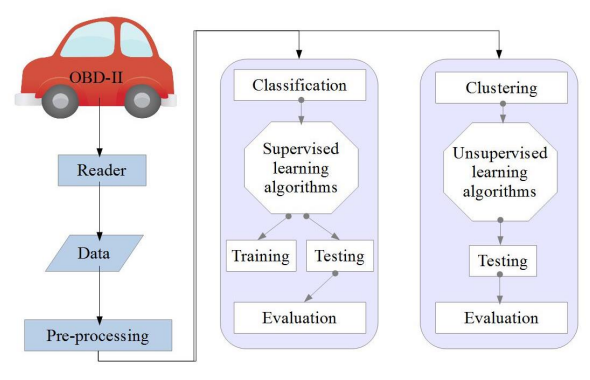
\includegraphics[width=.7\linewidth]{images/general-scheme-investigation.png}
  \caption{Esquema seguido para determinar los hábitos de conducción usando el \ac{OBD}--II \cite{hermawanAcquisitionModelingEvaluating2020}.}
  \label{fig:investigation-scheme}
\end{figure}

Por último, uno de los tipos de investigación bastante interesante realizada en los
últimos años es la de la generación de perfiles de conducción y de consumo. En el
artículo realizado por Ameen \textit{et al.} \cite{husseinaliameenDrivingBehaviourIdentification2021}
se define un sistema de clasificación del comportamiento del conductor al volante
(que es además el que se propone usar en este proyecto) el cual combina los datos
recibidos por el \ac{OBD}--II y del \ac{GPS} (figura \ref{fig:driving-behaviour}):

\begin{figure}[H]
  \centering
  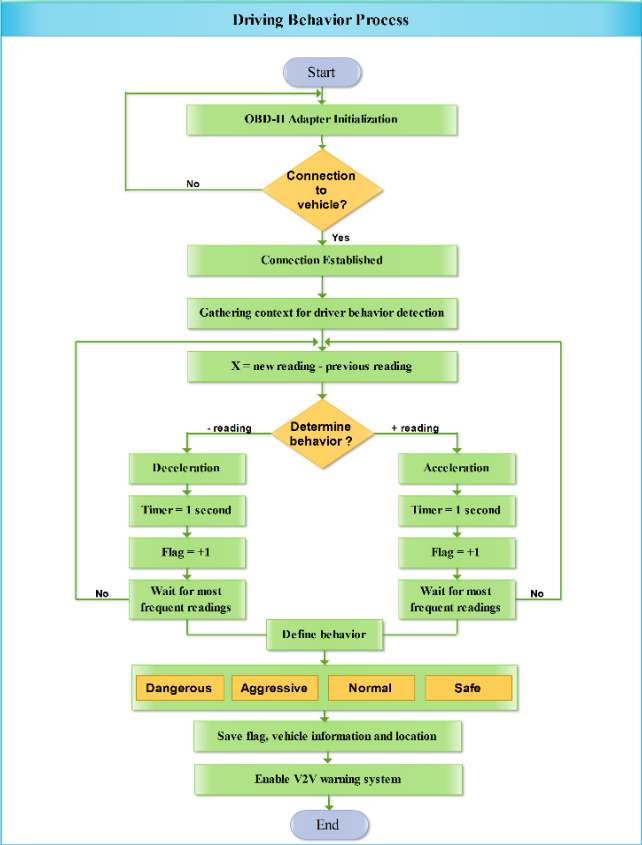
\includegraphics[width=.7\linewidth]{images/driving-behaviour-workflow.png}
  \caption{Flujo de análisis para determinar el comportamiento al volante de un conductor \cite{husseinaliameenDrivingBehaviourIdentification2021}.}
  \label{fig:driving-behaviour}
\end{figure}

Al final, el estudio concluía con los siguientes perfiles de conducción:

\begin{itemize}
  \item \textbf{Peligroso}, para una aceleración en general superior a $7\ \nicefrac{m}{s^2}$.
  \item \textbf{Agresivo}, para una aceleración entre $\left[4\ \nicefrac{m}{s^2}, 7\ \nicefrac{m}{s^2}\right)$.
  \item \textbf{Normal}, para una aceleración entre $\left[2\ \nicefrac{m}{s^2}, 4\ \nicefrac{m}{s^2}\right)$.
  \item \textbf{Seguro}, para una aceleración entre $\left[0\ \nicefrac{m}{s^2}, 2\ \nicefrac{m}{s^2}\right)$.
\end{itemize}
